This section covers the performance limitations of fusing several cores into a single logical core (LC).
This enables a better understanding of what leads to good performance and how to determine regions of code that benefit from core fusion.
The two major obstacles to gaining performance with core fusion are branch prediction and synchronization costs.

\subsection{Branch Prediction}

As discussed in the background chapter, DMPs accelerate a single thread by executing instructions from the same thread speculatively across several fused cores. 
Similarly, EDGE DMPs accelerate a single thread by speculatively executing instruction blocks~\cite{putnam2010e2}.
Core fusion puts a strain on the branch predictor since efficiently using the fused cores depends on the misprediction rate; this is due to the standard fetching scheme deployed by the DMP.
In a core composition, the fetching scheme dictates that a core must fetch blocks until its instruction window is full; once this requirement is met, the following block will then be sent to the next block in the composition.
The branch predictor has to meet a different accuracy requirement depending on the size of both the LC and average size of a block being executed.
Given a Logical Core \textit{LC} of size \textit{i}, denoted \textit{$LC_i$}, the minimum branch prediction requirement can be determined using Formula~\ref{form:minpred} where \textit{BlocksInFlight} represents the number of total blocks being executed on the \textit{LC}.
\begin{equation}\label{form:minpred}
min_{PredLC_i }= \frac{BlocksInFlight - 1}{BlocksInFlight}
\end{equation}

\textit{BlocksInFlight} will vary depending on the average size of the blocks, the maximum block size the architecture can execute (\textit{MaxBlockSize}), and the number of blocks 
that are allowed to execute in parallel on a physical core (\textit{NumOfBlocksPerCore}). 
The size of the instruction window is equivalent to \textit{MaxBlockSize} multiplied by \textit{NumOfBlocksPerCore}.
When a program is running on a LC, one of the blocks will always be unconditionally executed, which is why it requires one less block to be predicted.

Figure~\ref{fig:req_pred} shows the expected prediction accuracy required to fully utilize a LC given the average block size in flight.
In this figure, NumOfBlocksPerCore is equal to four and MaxBlockSize is 32.
Adding extra physical cores to a LC requires an increasingly accurate branch predictor, especially when the size of a block is under 50 instructions.
This informs us in two ways; first of all large LCs will need to run on code sections with less control flow as they are more sensitive to branch misspredictions.
Second of all, branch prediction can be a simple method of evaluating the current effectiveness of a LC.
Given a certain number of cores, if the prediction accuracy is under the limits presented in Figure~\ref{fig:req_pred} it can be easily determine that the LC is sub-optimal.

\begin{figure}[h]
    \centering
    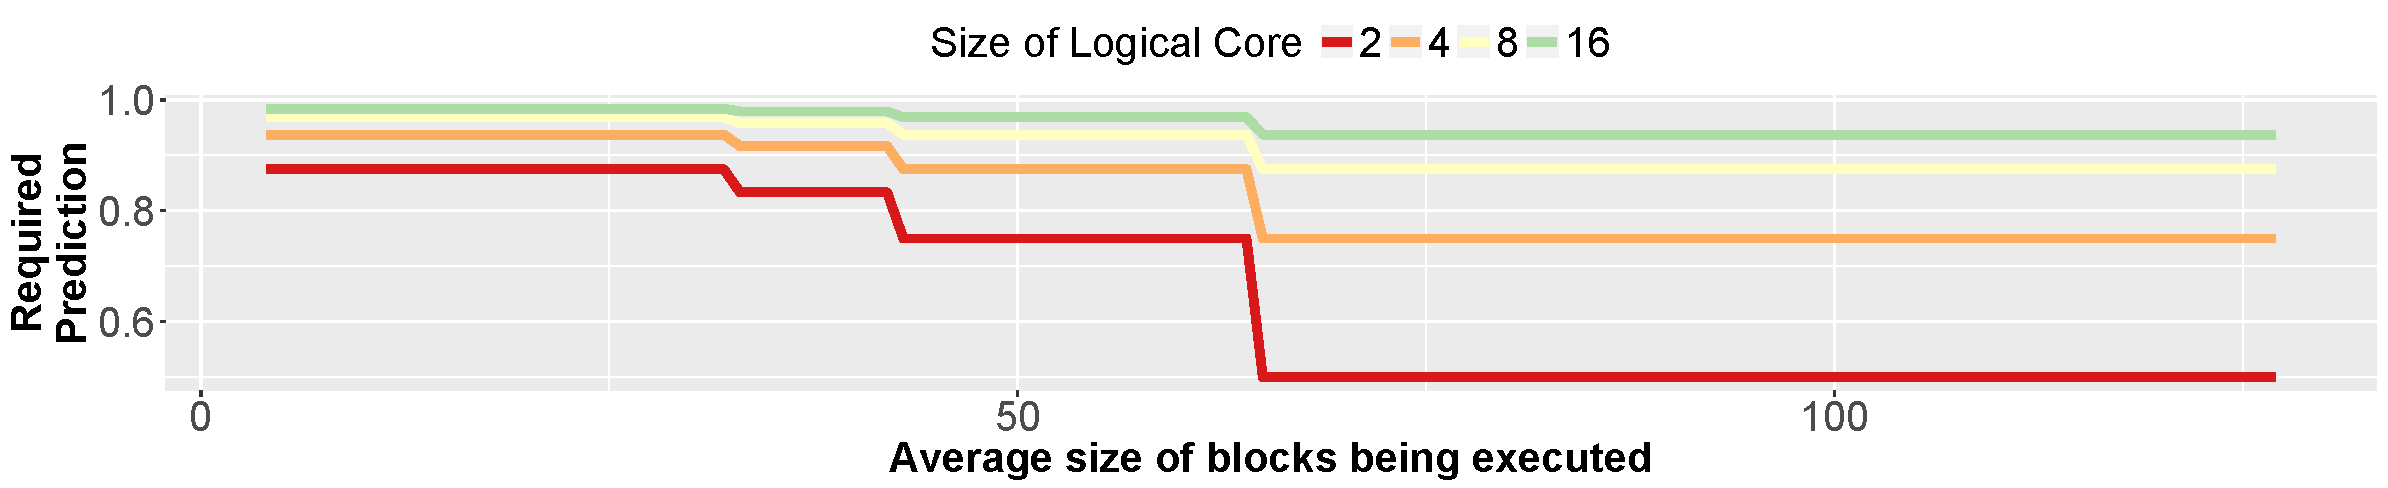
\includegraphics[width=\textwidth]{cases-paper/graphics/limit_study/prediction_req.pdf}
    \caption{Required prediction accuracy for a logical core size to be efficient given an average block size.}
    \label{fig:req_pred}
\end{figure}
\subsection{Synchronization Cost}

For a program to execute correctly, the cores in a logical core (LC) must communicate when they have finished executing a block. 
This ensures that the cores fetch blocks from the correct control paths and update memory and registers consistently.
A core may have to wait for other cores to commit before fetching a new block. 
The worst-case estimate of this stall is defined as the \textbf{Synchronization Cost}.

Blocks commit in a sequential fashion with the non-speculative block committing first and the most recent speculative block committing last.
If a core's instruction window is full then it must commit a block before it fetches a new one.
The Synchronization Cost, in cycles, is defined in equation~\ref{form:synccost} and is measured by averaging the overall number of cycles each fused core waits until it can continue to fetch and execute new blocks.
\textit{AvBlocksInFlight} represents the average number of blocks in flight on a single core in the LC.
This is a worst-case estimate as block sizes will fluctuate during the execution of a program.

\begin{equation}\label{form:synccost}
SyncCost_i = \frac{\sum_{n=0}^{i-1}\left(AvBlocksInFlight \right) \times n }{i}
\end{equation}


\begin{figure}[h]
    \centering
    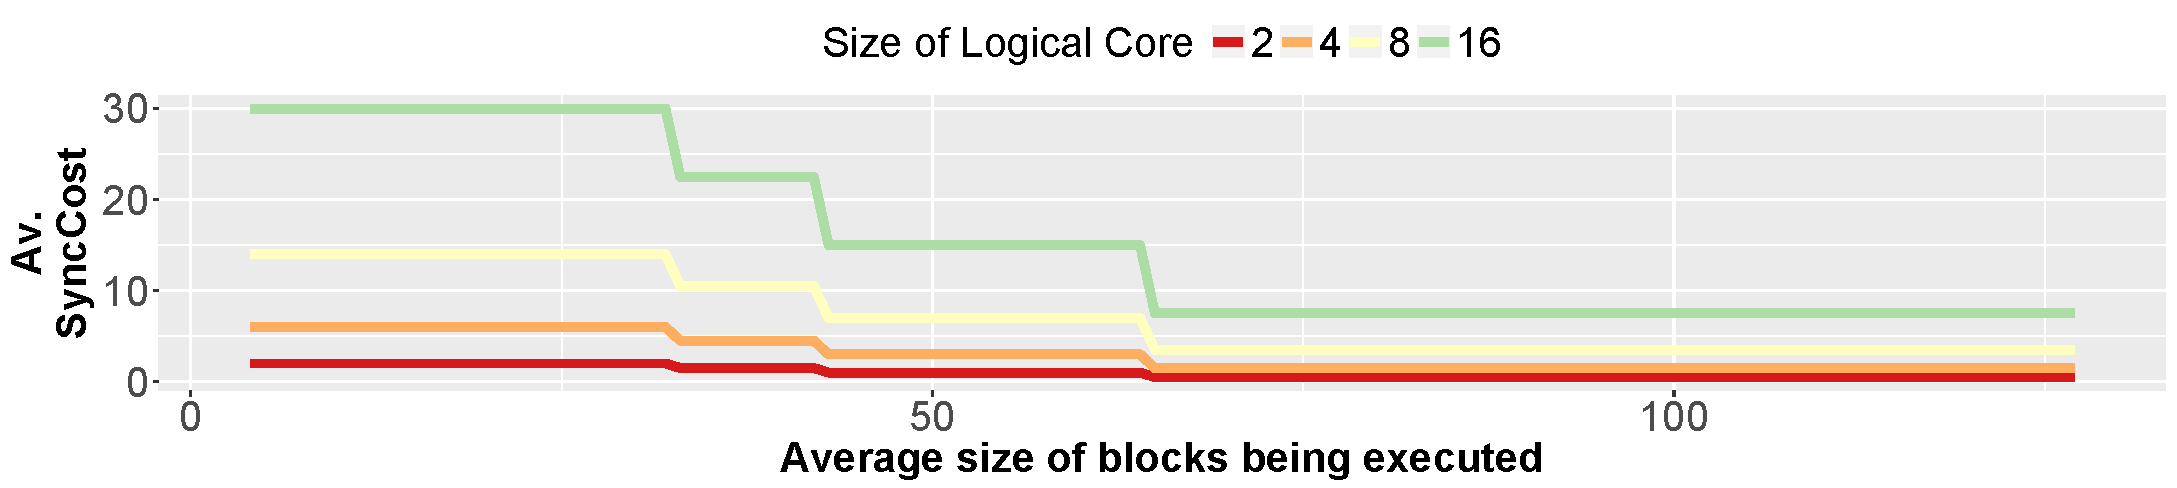
\includegraphics[width=\textwidth]{cases-paper/graphics/limit_study/sync_cost.pdf}

    \caption{Synchronization Cost in cycles for a given number of cores in a composition and an average block size.} %Each core has 4 lanes and each lane can fetch a block of up to 32 instructions. Lower is better.}
    \label{fig:sync_cost}
	\vspace{1em}
\end{figure}

Figure~\ref{fig:sync_cost} shows how many cycles the Synchronization Cost will be for a given LC and average block size.
The larger the block size the lower the Synchronization Cost is since cores fetch fewer blocks and wait less for other fused cores to finish committing.
Large LCs executing small blocks have a high Synchronization Cost. 
This indicates that large LCs should be avoided when dealing with smaller blocks as the Synchronization Cost outweighs the code execution.

\subsection{Summary}

This section estimated the worst-case IPC for a logical processor using Average Block Size, Average Branch Prediction, and Synchonization Cost.
Figure~\ref{fig:lm_summ} presented a worst-case estimate of IPC performance assuming each core can sustain an IPC of 2.
From what was previously explained, Figure~\ref{fig:lm_summ} shows us that to obtain optimal performance requires a high branch prediction accuracy and large blocks.
It shows that larger logical processors can easily under-perform; for example it can be seen that 16 fused cores often have IPCs under 15, meaning that each core has an IPC under~1.

\begin{figure}[t]
    \centering
    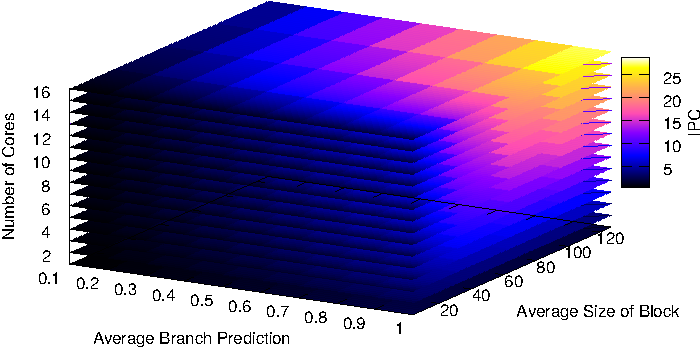
\includegraphics[width=0.8\textwidth]{cases-paper/graphics/limit_study/summary.pdf}
    \caption{IPC estimate given a logical processor size, average branch prediction and average block size for a dual-issue core. A higher IPC means better performance.}
    \label{fig:lm_summ}
\vspace{5mm}
\end{figure}
